\documentclass[12pt]{article}
\usepackage{graphicx,import}
\usepackage[svgnames]{xcolor} 
\usepackage{fancyhdr}
\usepackage{subfig}
\usepackage{hyperref}
\usepackage{enumitem}
\usepackage{cite}
\usepackage[many]{tcolorbox}
\usepackage{listings }
\usepackage[a4paper, total={6in, 8in} , bottom = 25mm , top = 25mm, headheight = 1.25cm , includehead,includefoot,heightrounded ]{geometry}
\usepackage{afterpage}
\usepackage{amssymb}
\usepackage{pdflscape}
\usepackage{gensymb}
\usepackage{textcomp}
\usepackage{tikz,pgfplots}
\usepackage{xecolor}
\usepackage{pgf,tikz}
\usetikzlibrary{arrows,automata}

\usepackage{rotating}
\usepackage{pdfpages}
\usepackage{fancyvrb}
\usepackage[Kashida]{xepersian}
\usepackage[T1]{fontenc}
\usepackage{tikz}
\usepackage[utf8]{inputenc}
\usepackage{PTSerif} 
\usepackage{seqsplit}

\usepackage[edges]{forest}

\usepackage{listings}
\usepackage{xcolor}

\hypersetup{
	colorlinks   = true, %Colours links instead of ugly boxes
	urlcolor     = blue, %Colour for external hyperlinks
	linkcolor    = blue, %Colour of internal links
	citecolor   = red %Colour of citations
}

\definecolor{codegreen}{rgb}{0,0.6,0}
\definecolor{codegray}{rgb}{0.5,0.5,0.5}
\definecolor{codepurple}{rgb}{0.58,0,0.82}
\definecolor{backcolour}{rgb}{0.95,0.95,0.92}

\NewDocumentCommand{\codeword}{v}{
	\texttt{\textcolor{blue}{#1}}
}
\lstset{language=java,keywordstyle={\bfseries \color{blue}}}

\lstdefinestyle{mystyle}{
	backgroundcolor=\color{backcolour},   
	commentstyle=\color{codegreen},
	keywordstyle=\color{magenta},
	numberstyle=\tiny\color{codegray},
	stringstyle=\color{codepurple},
	basicstyle=\ttfamily\normalsize,
	breakatwhitespace=false,         
	breaklines=true,                 
	captionpos=b,                    
	keepspaces=true,                 
	numbers=left,                    
	numbersep=5pt,                  
	showspaces=false,                
	showstringspaces=false,
	showtabs=false,                  
	tabsize=2
}

\lstset{style=mystyle}

\settextfont[Scale=1.2 ,BoldFont={Bahij Nazanin-Bold.ttf} , ItalicFont = {IRNazaninIranic.ttf}]{Bahij Nazanin-Regular.ttf}
\setlatintextfont[Scale = 1.0]{Garamond}
\DefaultMathsDigits 
\DeclareMathSizes{11}{19}{13}{9} 
%\DeclareMathSizes{12}{14.4}{8}{9}





\newenvironment{changemargin}[2]{%
	\begin{list}{}{%
			\setlength{\topsep}{0pt}%
			\setlength{\leftmargin}{#1}%
			\setlength{\rightmargin}{#2}%
			\setlength{\listparindent}{\parindent}%
			\setlength{\itemindent}{\parindent}%
			\setlength{\parsep}{\parskip}%
		}%
		\item[]}{\end{list}}


\definecolor{foldercolor}{RGB}{124,166,198}

\tikzset{pics/folder/.style={code={%
			\node[inner sep=0pt, minimum size=#1](-foldericon){};
			\node[folder style, inner sep=0pt, minimum width=0.3*#1, minimum height=0.6*#1, above right, xshift=0.05*#1] at (-foldericon.west){};
			\node[folder style, inner sep=0pt, minimum size=#1] at (-foldericon.center){};}
	},
	pics/folder/.default={20pt},
	folder style/.style={draw=foldercolor!80!black,top color=foldercolor!40,bottom color=foldercolor}
}

\forestset{is file/.style={edge path'/.expanded={%
			([xshift=\forestregister{folder indent}]!u.parent anchor) |- (.child anchor)},
		inner sep=1pt},
	this folder size/.style={edge path'/.expanded={%
			([xshift=\forestregister{folder indent}]!u.parent anchor) |- (.child anchor) pic[solid]{folder=#1}}, inner xsep=0.6*#1},
	folder tree indent/.style={before computing xy={l=#1}},
	folder icons/.style={folder, this folder size=#1, folder tree indent=3*#1},
	folder icons/.default={12pt},
}

\begin{document}
	
	
	%%% title pages
	\begin{titlepage}
		\begin{center}
			
			\vspace*{0.7cm}
			
			
\includegraphics[width=0.4\textwidth]{sharif1.png}\\
			\vspace{0.5cm}
			\textbf{ \Huge{\emph  ﺷﺒﻜﻪ‌های کامپیوتری} }\\
			\vspace{0.5cm}
			\textbf{ \Large{ تمرین سوم} }
			\vspace{0.2cm}
			
			
			\large \textbf{دانشکده مهندسی کامپیوتر}\\\vspace{0.2cm}
			\large   دانشگاه صنعتی شریف\\\vspace{0.2cm}
			\large   ﻧﯿﻢ سال دوم 00-99 \\\vspace{0.2cm}
			\noindent\rule[1ex]{\linewidth}{1pt}
			استاد:\\
			\textbf{{جناب آقای دکتر جعفری}}
			
			
			\vspace{0.15cm}
			نام و نام خانوادگی:\\
			
			
			\textbf{{امیرمهدی نامجو - 97107212}}
		\end{center}
	\end{titlepage}
	%%% title pages
	
	
	%%% header of pages
	\newpage
	\pagestyle{fancy}
	\fancyhf{}
	\fancyfoot{}
	\cfoot{\thepage}
	\chead{تمرین سوم}
	\rhead{
\includegraphics[width=0.1\textwidth]{sharif.png}}
	\lhead{امیرمهدی نامجو}
	%%% header of pages
	
	\KashidaOff
	
	\section{سوال اول}


روش \lr{UDP Hole Punching} روشی است که به کمک آن می‌توان ارتباط بین دو کلاینت که یک یا هر دوی آن ها پشت \lr{NAT} قرار دارند را برقرار کرد. در اصل این روش به نوعی یک حفره در دیواره \lr{NAT} ایجاد می‌کند و برای همین \lr{Hole Punching} نام دارد. نحوه کار این روش بدین صورت است:

فرض کنید می‌خواهیم ارتباط بین \lr{A} و \lr{B} را برقرار کنیم. در روش \lr{Hole Punching} نیاز به داشتن یک واسطه مانند \lr{C} است که هر دوی \lr{A} و \lr{B} آدرس \lr{IP} آن را بداند.

در مرحله اول \lr{A} و \lr{B} هر دو پکت‌های \lr{UDP} را به \lr{C} می‌فرستند. با عبور پکت های آنان از \lr{NAT} شان، این \lr{NAT}، آدرس \lr{IP} مبدا این پکت‌ها را بازنویسی می‌کند تا مشخص باشد که پاسخ آن باید به کجا ارسال شود.

در مرحله دوم، \lr{C} متوجه \lr{IP} آدرس و همچنین پورت درخواست هایی که از سمت \lr{A} و \lr{B} آمده‌اند می‌شود. (مثلا فرض کنید پورت \lr{A} برابر \lr{X} و پورت \lr{B} برابر \lr{Y } باشد) با توجه به ساختار عمومی \lr{NAT}، در حال حاضر \lr{C} می‌تواند به راحتی از این طریق با \lr{A} و \lr{B} ارتباط برقرار کند و با ارسال پیام به \lr{NAT} هر کدام از آن‌ها، از آن جایی که \lr{NAT} می‌داند که شروع درخواست از سمت قسمت‌های درونی خود بوده است و اطلاعات را دارد، بسته را به درستی به مقصد می‌رساند.

در مرحله بعد، \lr{C} به \lr{A} پیامی می‌دهد که می گوید برای ارتباط برقرار کردن با \lr{B}، برای آدرس \lr{IP} مربوط به \lr{NAT} آن و پورت \lr{Y} پیام ارسال کن. از طرفی به \lr{B }هم می‌گوید برای ارتباط برقرار کردن با \lr{A} به آدرس \lr{IP} مربوط به \lr{NAT} آن و پورت \lr{X} پیام ارسال کن.

در مرحله بعد، ابتدا اولین پکت های ارسالی از سمت \lr{A} و \lr{B} به درستی به مقصد نمی رسد و توسط \lr{NAT}های مربوطه \lr{Reject} می‌شود. اما با ارسال اولین پیام از سمت \lr{A} به \lr{B} و عبور آن از \lr{NAT} مربوط به \lr{A}، این \ lr{NAT}متوجه می‌شود که \lr{A} قصد ارتباط برقرار کردن با \lr{IP} آدرسی که مربوط به \lr{NAT} هاست \lr{B} است و پورت \lr{Y} را دارد و از این رو پیام های دریافتی بعدی از این آردس را برای \lr{A} می فرستد. همین اتفاق از سمت \lr{NAT} دیگر هم می افتد. از این به بعد این دو \lr{NAT} می‌دانند درخواست‌هایی که از سمت مقابل می‌آید را باید به کدام یک از \lr{Host} های سمت خود تحویل بدهند. به نوعی یک حفره در \lr{NAT} ایجاد شده که درخواست‌هایی که از آدرس خاصی می‌آیند را به درستی به یکدیگر تحویل می‌دهد. بدین ترتیب ارتباط \lr{P2P} بین \lr{A} و \lr{B} برقرار می‌شود.


در اصل اگر بخواهیم به صورت دقیق تر توضیح بدهیم به شکل زیر می شود (مطابق توضیحات ویکیپدیا):

\begin{enumerate}
	\item 
	هر کدام از \lr{A} و \lr{B} ارتباط \lr{UDP} را با \lr{C} شروع می کنند. \lr{NAT} های هر کدام یعنی \lr{NA} و \lr{NB} دو پورت خارجی موقت \lr{EPA} و \lr{EPB} را به این کار اختصاص می دهند.
	
	\item
	\lr{C} 
	بسته های دریافتی را بررسی  می کند تا آدرس \lr{IP} هر کدام از \lr{NAT} ها و همچنین \lr{EPA} و \lr{EPB} را بیابد.
	\item
	\lr{C}
	پیامی حاوی \lr{EIPA:EPA} را به \lr{B} و پیامی حاوی \lr{EIPB:EPB} را به \lr{A} می فرستد.
	
	\item
	\lr{A}
	یک بسته به \lr{EIPB:EPB} می فرستد.
	
	\item
	\lr{NAT}
	هاست A بررسی بسته را بررسی می کند و در جدول ترجمه اش قرار می دهد:
	
	\lr{(Source-IP-A , EPA, EIPB , EPB)}
	
	که بداند پیام های دریافتی از \lr{B } را باید به کجا بفرستد.
	
	\item
\lr{B}
یک بسته به \lr{EIPA:EPA} می فرستد.

\item
\lr{NAT}
هاست \lr{B} بررسی بسته را بررسی می کند و در جدول ترجمه اش قرار می دهد:

(\lr{Source-IP-B} , \lr{EPB}, \lr{EIPA} , \lr{EPA})

که بداند پیام های دریافتی از \lr{A} را باید به کجا بفرستد.


\item
بسته به وضعیت \lr{NAT} هاست \lr{A} که در هنگام دریافت بسته \lr{B}، داده مربوط به آن را در جدول ترجمه‌اش نوشته باشد یا نه، بسته اول دریافتی از \lr{B} یا رد می‌شود و یا دریافت می‌شود.



\item
بسته به وضعیت \lr{NAT} هاست \lr{B} که در هنگام دریافت بسته \lr{A}، داده مربوط به آن را در جدول ترجمه اش نوشته باشد یا نه، بسته اول دریافتی از \lr{A} یا رد می شود و یا دریافت می شود.


\item

در بدترین حالت، هر دو دومین بسته ای که از سمت دیگری می آید را دریافت کرده و ارتباط برقرار می شود.



به طور کلی این روش امروزه هم در ارتباطات \lr{P2P} و همچنین \lr{VoIP} استفاده می‌شود. با این حال باید چند نکته را در نظر داشت. بعضی از \lr{NAT} ها در هر بار ارتباط آدرس پورت را عوض می‌کنند. یعنی حتی اگر پورت و \lr{IP} مبدا هم یکی باشد، با متفاوت شدن مقصد ها پورت های متفاوتی روی \lr{NAT} به آن ها اختصاص می یابد. این موضوع در \lr{Symemetric NAT} ها وجود دارد و باعث ایجاد مشکل در این تکنیک می شود.

مشکل دیگری که ممکن است پیش بیاید، این است که یک سیستم پشت چند سطح مختلف از \lr{NAT} ها باشد. در این موارد ممکن است یکی از \lr{NAT} های لایه بالاتر که به تعداد خیلی زیادی سرویس خدمت رسانی می کند، \lr{Port} ها را تغییر بدهد و بدون نیاز دائمی به واسط \lr{C} نتوان ارتباط درست \lr{P2P} برقرار کرد.

همچنین یک چالش دیگر زمانی پیش می آید که هر دو سیستم پشت یک \lr{NAT} باشند. در این مواقع بعضی از \lr{NAT} ها درخواستی که برای خودشان آمده باشد و \lr{Loopback} به درون سیستم باشد را به درستی جواب نمی دهند. برای رفع این مشکل، معمولا به این شکل عمل می شود که اطلاعات \lr{IP} و \lr{Port} خصوصی که در ابتدا Host های اولیه قرار داده‌اند هم از طریق واسط به دیگری فرستاده می‌شود تا سعی کند از طریق شبکه داخلی هم ارتباط برقرار کند و اگر هر دو متوجه شدند پشت یک \lr{NAT} هستند صرفا از طریق شبکه داخلی ارتباط را برقرار کنند و دیگر به آدرس \lr{IP} و \lr{Port} عمومی \lr{NAT} که از بیرون قابل مشاهده بوده چیزی ارسال نکنند.

روش کار \lr{Skype} بدین صورت است که از طریق پروتکل هایی نظیر \lr{STUN} یا \lr{ICE} متوجه وضعیت \lr{NAT} هر کدام از کاربرها می‌شود. تعدادی از کاربران هستند که پشت \lr{NAT} نیستند و \lr{IP} عمومی قابل دسترس دارند. این کاربران به نوعی در نقش واسط هایی عمل می‌کنند که در روش \lr{Hole Punching} ارتباط بین دو Host دیگر را برقرار می‌کردند. با توجه به این موضوع خود \lr{Skype} نیاز دارد که بداند چه کاربرانی پشت \lr{NAT} هستند و چه کاربرانی نیستند.

در صورتی که به دلیل ساختار خاص \lr{NAT} یکی از کاربران نظیر عوض کردن پورت در سیستم \lr{Symmetric}  به هیچ وجه امکان \lr{UDP Hole Punching} مهیا نباشد، عملا آن کاربر واسط، تبدیل به نوعی سرور میانی می شود که ارتباط میان دو کاربری که قصد ارتباط برقرار کردن را داشتند را بین آن ها جا به جا می کند. یعنی در این حالت دیگر این واسط، فقط برای ارتباط برقرار کردن اولیه استفاده نمی‌شود، بلکه همه پیام ها باید یک بار به دست آن واسط رسیده و بعد برای مقصد اصلی ارسال بشوند.

البته در کنار همه این ها باید توجه کرد که یکسری \lr{Login Server} هم وجود دارد که مقوله آن ها مستقل از برقراری ارتباط است و برای احراز هویت اولیه است. بدیهتا این سرورها به صورت متمرکز در دیتاسنترهای مایکروسافت قرار دارد و اطلاعات احراز هویت دست کاربران مختلف نیست.

همچنین باید به یک نکته دیگر هم توجه کرد و آن هم این که هر چند در پروتکل اولیه استفاده شده توسط \lr{Skype}، هر کاربری که پشت \lr{NAT} نبود می توانست در نقش سرورهای برقرارکننده ارتباط قرار بگیرد، اما این موضوع باعث نارضایتی برخی کاربران شده بود که از آن ها به دلیل محدودیت کمتر اینترنتشان و قرار نداشتن پشت \lr{NAT} به عنوان واسط برقراری ارتباط میان دو کاربر دیگر استفاده می‌شود. به همین علت بعد از خریداری شدن \lr{Skype} توسط مایکروسافت، تقریبا همه این \lr{Supernode} ها که وظیفه ارتباط برقرار کردن بین کاربران را دارند، متشکل از سرورهای اختصاصی قرار گرفته در دیتاسنترهای مایکروسافت هستند و از کاربران برای برقراری \lr{UDP Hole Punching} استفاده نشده و این وظیفه برعهده سرورهای اختصاصی مایکروسافت است.


در مورد این که آیا نیاز به اطلاع از وجود \lr{NAT} داریم یا نه، می توان هم جواب بله داد و هم خیر. به طور کلی خود عملیات \lr{UDP Hole Punching} مستقل از وجود یا عدم وجود \lr{NAT} در دو سیستمی که قصد ارتباط برقرار کردن دارند، قابل اجراست و در روند انجام فرآیند تغییری ایجاد نمی‌شود. با این حال، به هر حال مسئله پیدا کردن شخص ثالث واسط وجود دارد. در سیستمی نظیر \lr{Skype}، تا قبل از متمرکز شدن سرورها در دیتاسنترهای مایکروسافت، شخص ثالث واسط هم از کاربران بود و برای پیدا کردن چنین فردی، نیاز به پروتکل‌های پیمایش \lr{NAT} بود تا مطمئن بشویم که این فرد پشت \lr{NAT} نیست و به طور مستقیم \lr{IP} عمومی دارد. همچنین در مواقعی که چندین لایه \lr{NAT} وجود دارد، ممکن است به دلیل نحوه تنظیم \lr{NAT}‌ ها عملا به طور کلی \lr{UDP Hole Punching} امکان پذیر نباشد و نیاز باشد که سرور واسط، تمامی پیام‌ها را بین دو \lr{endpoint} جا به جا کند. در چنین حالاتی، نیاز به دانستن ساختار شبکه و این که \lr{NAT} وجود دارد یا نه و به چه صورتی تنظیم شده است وجود دارد. در نتیجه هر چند خود نحوه انجام عملیات برای سیستمی که پشت \lr{NAT} هست یا نه تفاوت چشمگیری ندارد، اما در یک نرم افزار نظیر \lr{Skype} که قصد پیدا کردن واسطه‌ها را دارد و همین طور می‌خواهد در سختگیرانه‌ترین تنظیمات \lr{NAT} هم بتواند سرویس‌دهی کند، نیاز به دانستن این موضوع دارد.



در مورد محدودیت‌های این تکنیک، ابتدا باید به این نکته اشاره کرد که همان طور که گفته شد، اگر \lr{NAT} به صورت \lr{Symmetric} باشد، عملا امکان انجام این کار وجود ندارد. به علاوه این شیوه متکی بر وجود یک سیستم ثالث است که ارتباط دهی اولیه را برقرار کند و در نتیجه نیاز به نوعی پروتکل یا سرور مرکزی هست که این واسطه‌ها را پیدا‌ کند. مسئله دیگر در این است که به هر حال در این شیوه روی سیستم‌های واسطه فشار وارد می‌شود و عملا خود آن‌ها از این لود وارد شده، منفعت و سودی نمی‌برند. همین موضوع باعث اعتراض برخی کاربران \lr{Skype} هم شده بود و در نهایت بعد از خریداری آن توسط مایکروسافت، این سرورهای واسطه هم به دیتاسنترهای مایکروسافت منتقل شدند. علاوه بر این طول عمر اتصالات \lr{UDP} معمولا خیلی طولانی نیست و در نتیجه باید پکت‌های \lr{Keep-Alive} ارسال بشود که از بسته نشدن اتصال اطمینان حاصل بشود. چون در صورت بسته شدن اتصال عملا ممکن است جدول ترجمه \lr{NAT} هم دچار تغییر باشد و در نتیجه دوباره نیاز به انجام فرآیند \lr{UDP Hole Punching} باشد.


منابع استفاده شده برای پاسخ این سوال:

 \href{https://en.wikipedia.org/wiki/Hole_punching_(networking)}{ویکی‌پدیا}, \href{https://en.wikipedia.org/wiki/Network_address_translation}{ویکی‌پدیا }, \href{https://resources.infosecinstitute.com/topic/udp-hole-punching/}{\lr{Infosec}} و \href{https://bford.info/pub/net/p2pnat/}{\lr{bford.info}}
 
\end{enumerate}

\newpage
\section{سوال دوم}

\subsection{الگوریتم ساده}

\subsubsection{\lr{Link State}}

جدول آن به صورت زیر می‌شود. در ستون‌های مربوط به هر کدام از Node ها عدد اول مربوط به کمترین هزینه تا آن Node و عدد دوم مربوط به Parent آن Node است که با استفاده از آن این کمترین هزینه حاصل می‌شود.

\begin{center}
	\begin{latin}
		\begin{table}[h!]
			\centering
			\resizebox{\textwidth}{!}{%
				\begin{tabular}{|c|c|c|c|c|c|}
					\hline
					\textbf{Step} & \textbf{N'}    & \textbf{R2}                 & \textbf{R3}                 & \textbf{R4}                 & \textbf{R5}                 \\ \hline
					0             & R1             & 6,R1                        & 2,R1                        & {\color[HTML]{FE0000} 1,R1} & $\infty$      \\ \hline
					1             & R1,R4          & 3,R4                        & {\color[HTML]{FE0000} 2,R1} & -                           & 4,R4                        \\ \hline
					2             & R1,R4,R3       & {\color[HTML]{FE0000} 3,R4} & -                           & -                           & 4,R4                        \\ \hline
					3             & R1,R4,R3,R2    & -                           & -                           & -                           & {\color[HTML]{FE0000} 4,R4} \\ \hline
					4             & R1,R4,R3,R2,R5 & -                           & -                           & -                           & -                           \\ \hline
				\end{tabular}%
			}
		\end{table}
	\end{latin}
\end{center}

مقادیر نهایی به صورت زیر می‌شود:

$$D_{R1}(R2) , P_{R1}(R2) = 3 , R4$$


$$D_{R1}(R3) , P_{R1}(R3) = 2 , R1$$


$$D_{R1}(R4) , P_{R1}(R4) = 1 , R1$$


$$D_{R1}(R5) , P_{R1}(R5) = 4 , R4$$



\subsubsection{\lr{Dsitance Vector}}

برای این سوال فرض را بر این می‌گذاریم که در ابتدای کار و تا مرحله استیبل شدن مسیریاب ۵ به درستی 
کار کرده باشد و بعد غیرفعال شده باشد. چون اگر از ابتدای کار کلا غیرفعال باشد که مانند این است که اصلا حذف شده باشد و از آن جایی که همچنان بقیه متصل هستند، مشکل خاصی پیش نمی‌آید.

اگر به توپولوژی داده شده دقت کنیم، می بینیم که ۵ فقط با ۲ و ۴ در ارتباط است. بقیه هیچ کدام مستقیما با 5 در ارتباط نیستند. از طرف دیگر، ارتباط داشتن 5 با ۲ و۴ باعث نمی‌شود که تغییری در فاصله کمینه ای که این دو از هم در نظر دارند اتفاق بیفتد. زیرا فاصله این دو از هم ۲ است ولی اگر بخواهند از ۵ استفاده کنند فاصله ۴ می شود. در نتیجه ۵ اثری روی فاصله این دو هم نخواهد گذاشت. در نتیجه در تمامی مراحل بردار فاصله که اطلاعات بین مسیریاب ها رد و بدل می شود، اطلاعات ۵ اثری روی کمینه فاصله ای که بقیه نسبت به هم دارند نخواهد گذاشت. یعنی ۵ به جز مسیرهایی که به خودش منتهی می شود، در هیچ مرحله‌ای در هیچ مسیر کمینه‌ای نیست. در نتیجه در هر مرحله‌ای که این مسیریاب به مشکل بخورد، به جز این که بدیهتا مسیریابی به خود آن دچار مشکل می‌شود، برای بقیه مسیرها هیچ مشکلی پیش نمی‌آید.


پس در این مورد خاص مشکلی پیش نیامد. اما فرض کنیم که واقعا خرابی ۵ باعث مشکل در مسیر می‌شد. باید راهکار را برای این حالت بررسی کنیم. با خرابی ۵ در ابتدا ممکن است بقیه فکر کنند که چون تغییری در بردارهای مربوط به آن ایجاد نشده پیامی نمی‌آید. اما به هر حال  در یک مرحله‌ای یکی از مسیریاب‌های متصل به 5 (مثلا با نام A) یا سعی‌ می‌کند بردار آپدیت شده خود را به ۵ بفرستد یا این که سعی می‌کند که داده‌ای که به مقصد ۵ است را به آن بفرستد. در این زمان متوجه می‌شود که ۵ پاسخگو نیست. در این حالت می‌تواند وزن مربوط به ۵ را در بردار خود بی نهایت قرار بدهد. البته باید توجه کرد که اگر چند گره دیگر هم به ۵ مسیر داشته باشند (مانند همین توپولوژی سوال)، ممکن است گره ما فرض کند شاید فقط لینک خودش خراب شده است و سعی کند از طریق بقیه انتقال را انجام دهد. در این حالت نیز \lr{Poisoned Reverse} چاره کار خواهد بود. یعنی می‌تواند سعی‌کند از طریق گره‌های دیگری که به ۵ متصل هستند این کار را انجام دهد ولی حداقل به همان گره‌ که از طریق آن مسیریابی را انجام می‌دهد، اعلام می‌کند که فاصله خودش تا ۵ بی نهایت است که گره دوم سعی نکند از طریق خود A مسیریابی به ۵ انجام بدهد. بدین ترتیب به تدریج گره‌های دیگری که به 5 متصل بودند هم متوجه می‌شوند که امکان ارتباط با ۵ را ندارند. 

یک راه بهتر برای رفع مشکل هم این است که صرفا منتظر نباشیم که ببینیم چه زمانی پیامی به مقصد ۵ می‌آید و آن زمان وضعیت ۵ را چک کنیم. بلکه همه گره‌ها مستقل از پیام معمول آپدیت بردارها و پیام‌هایی که بنا بر وظیفه جا به جا می‌کنند، در بازه‌های زمانی مشخص به گره‌های همسایه خود از طریق لینک مربوطه، یکسری پیام Hello به یکدیگر بفرستند تا مطمئن شوند که لینک و گره دیگر سالم است و در صورتی که دیدند پاسخی دریافت نمی‌شود، سعی‌ کنند مسیریابی را از طریق یکی دیگر از همسایه‌های خود به آن لینک انجام دهند و به آن همسایه‌ هم اعلام کنند که مسیرشان تا گره احتمالا شکست خورده بی‌نهایت است که دور پیش نیاید. بدین ترتیب با ضریب اطمینان بیش‌تری مطمئن خواهیم بود که بعد از مدت زمان تعیین شده و کوتاهی، همگی متوجه خرابی آن گره خواهند شد. در حالت قبلی تا زمانی که نیازی به ارسال پیام به آن گره احساس نمی‌شد، متوجه خرابی آن نمی‌شدیم ولی در این روش که به صورت دوره‌ای همه گره‌ها و لینک‌ها چک می‌شوند، در صورت خرابی یک گره به سرعت همگی متوجه خواهند شد.

 
 در کل بهترین روش ترکیبی از Poisoned Reverse و خبر گرفتن هر گره از همسایه‌هایش در بازه‌های زمانی مشخص است که از فیل شدن لینک (و احتمالا خود گره) مطمئن شویم.
 
 
 در صفحه بعد مراحل اجرای الگوریتم (بدون در نظر گرفتن Poisoned Reverse) قرار دارند. مرحله بعدی درست مشابه مرحله آخر خواهد بود و بدین دلیل دوباره نوشته نشده است. (مراحل با فرض فیل نشدن ۵ رسم شده‌اند تا نشان داده شود که ۵ تاثیری در مسیرهای پیدا شده ندارد) 
 
 \newpage
 \begin{center}
 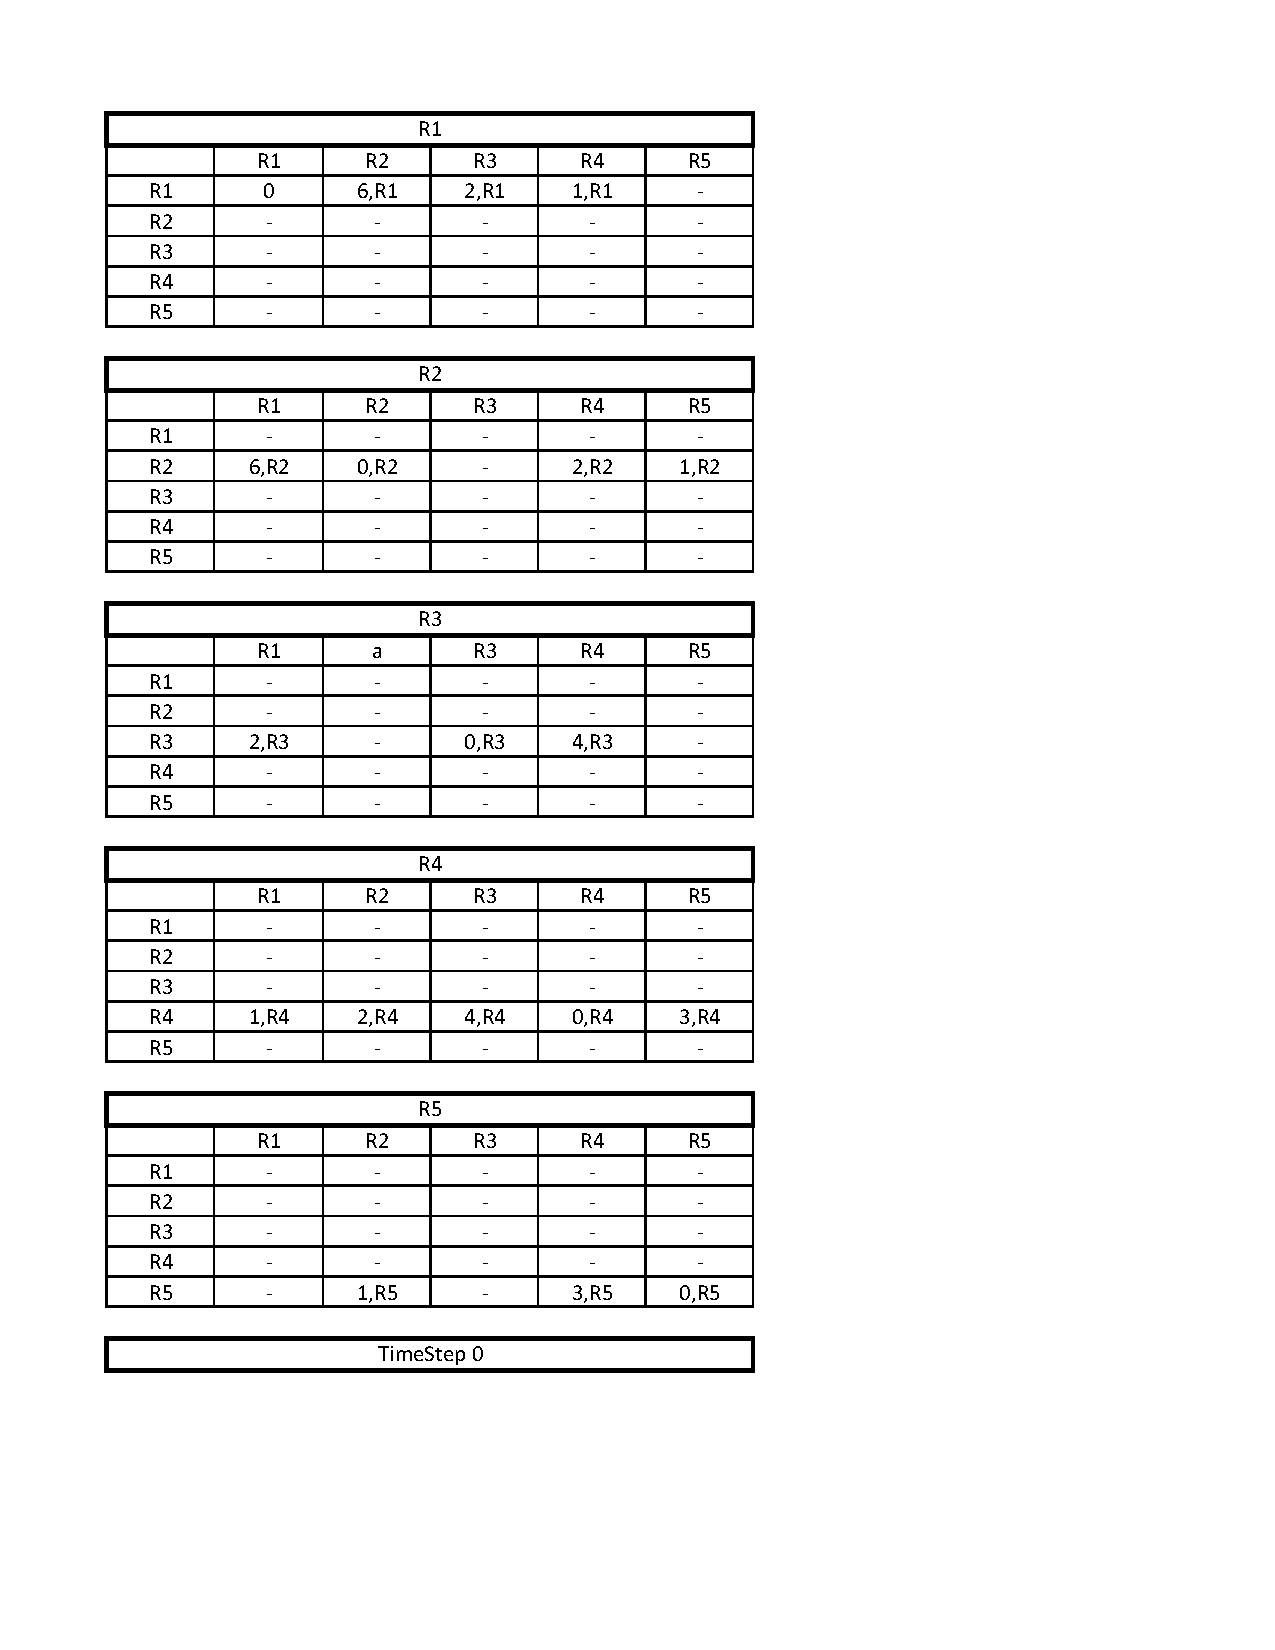
\includegraphics[width = 1.0 \textwidth]{images/1.pdf}
 \end{center}


 \begin{center}
	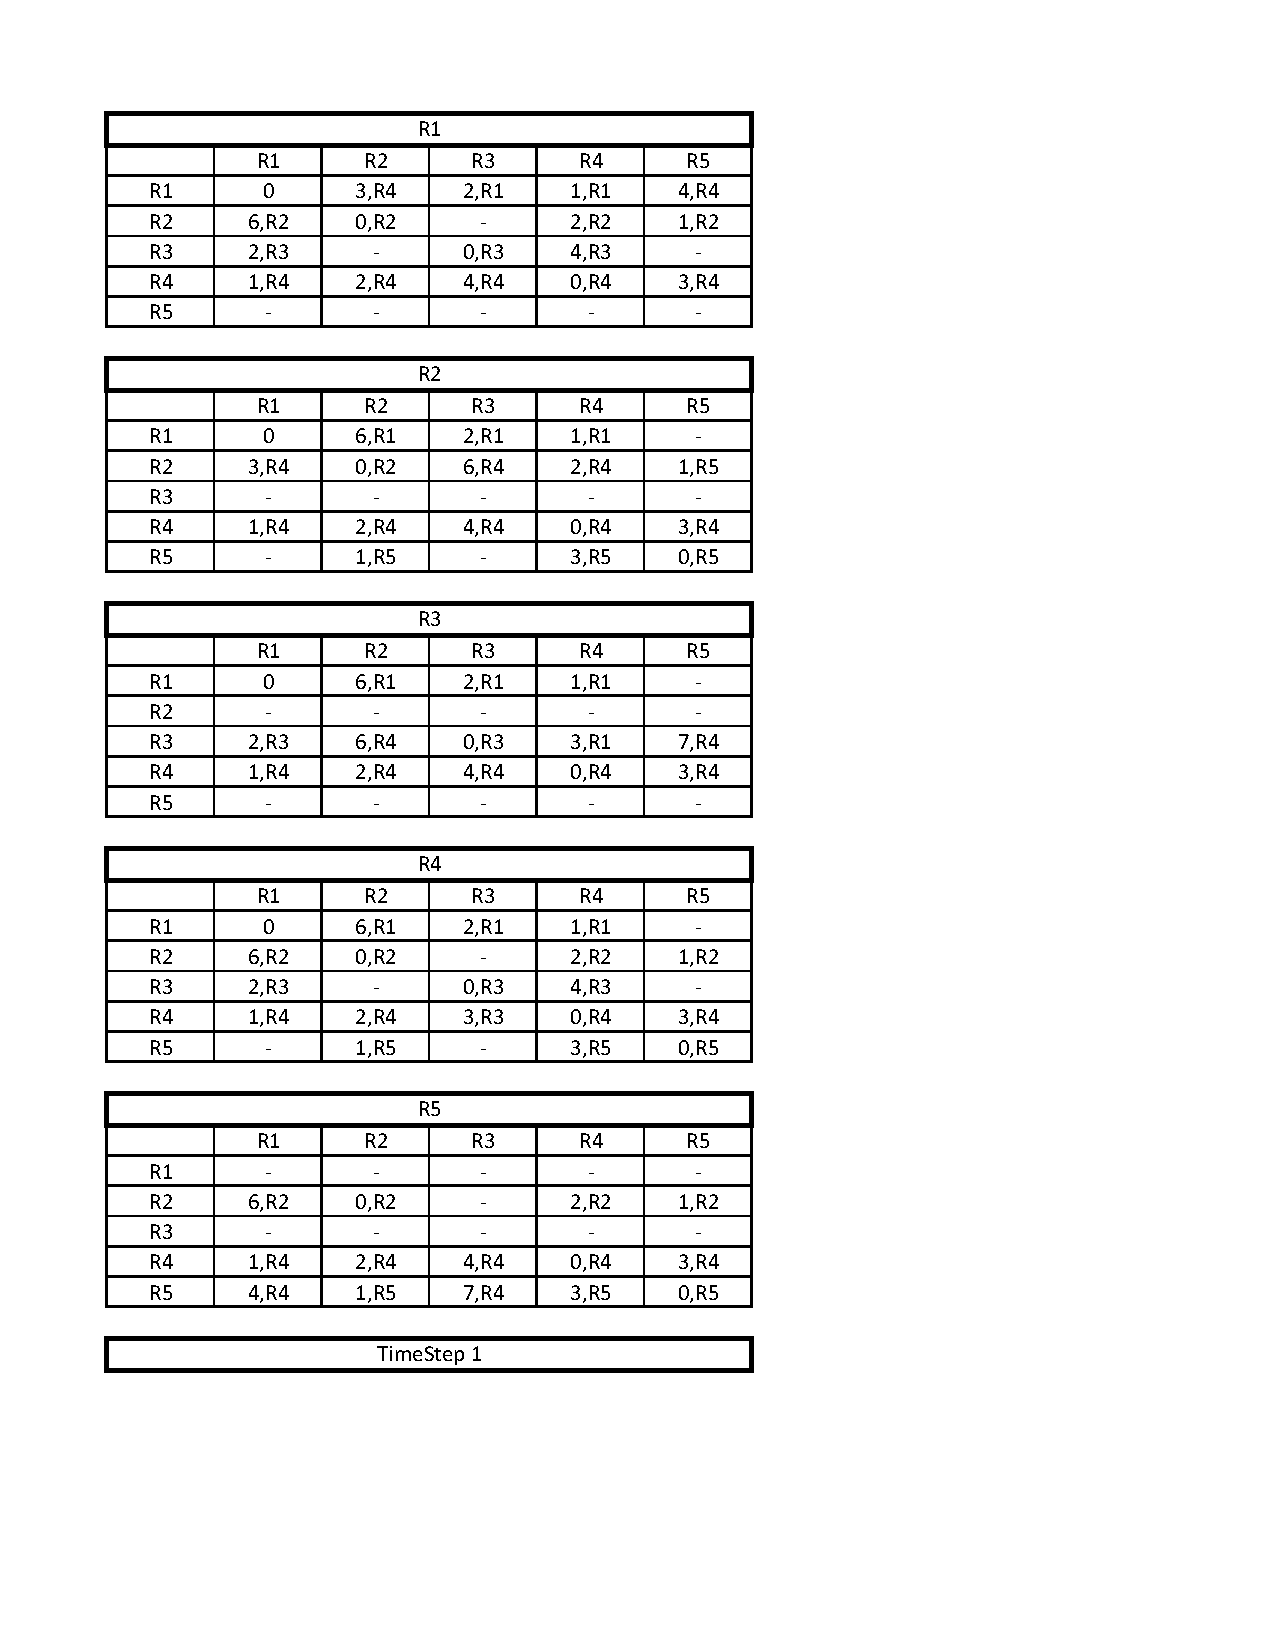
\includegraphics[width = 1.0 \textwidth]{images/2.pdf}
\end{center}



 \begin{center}
	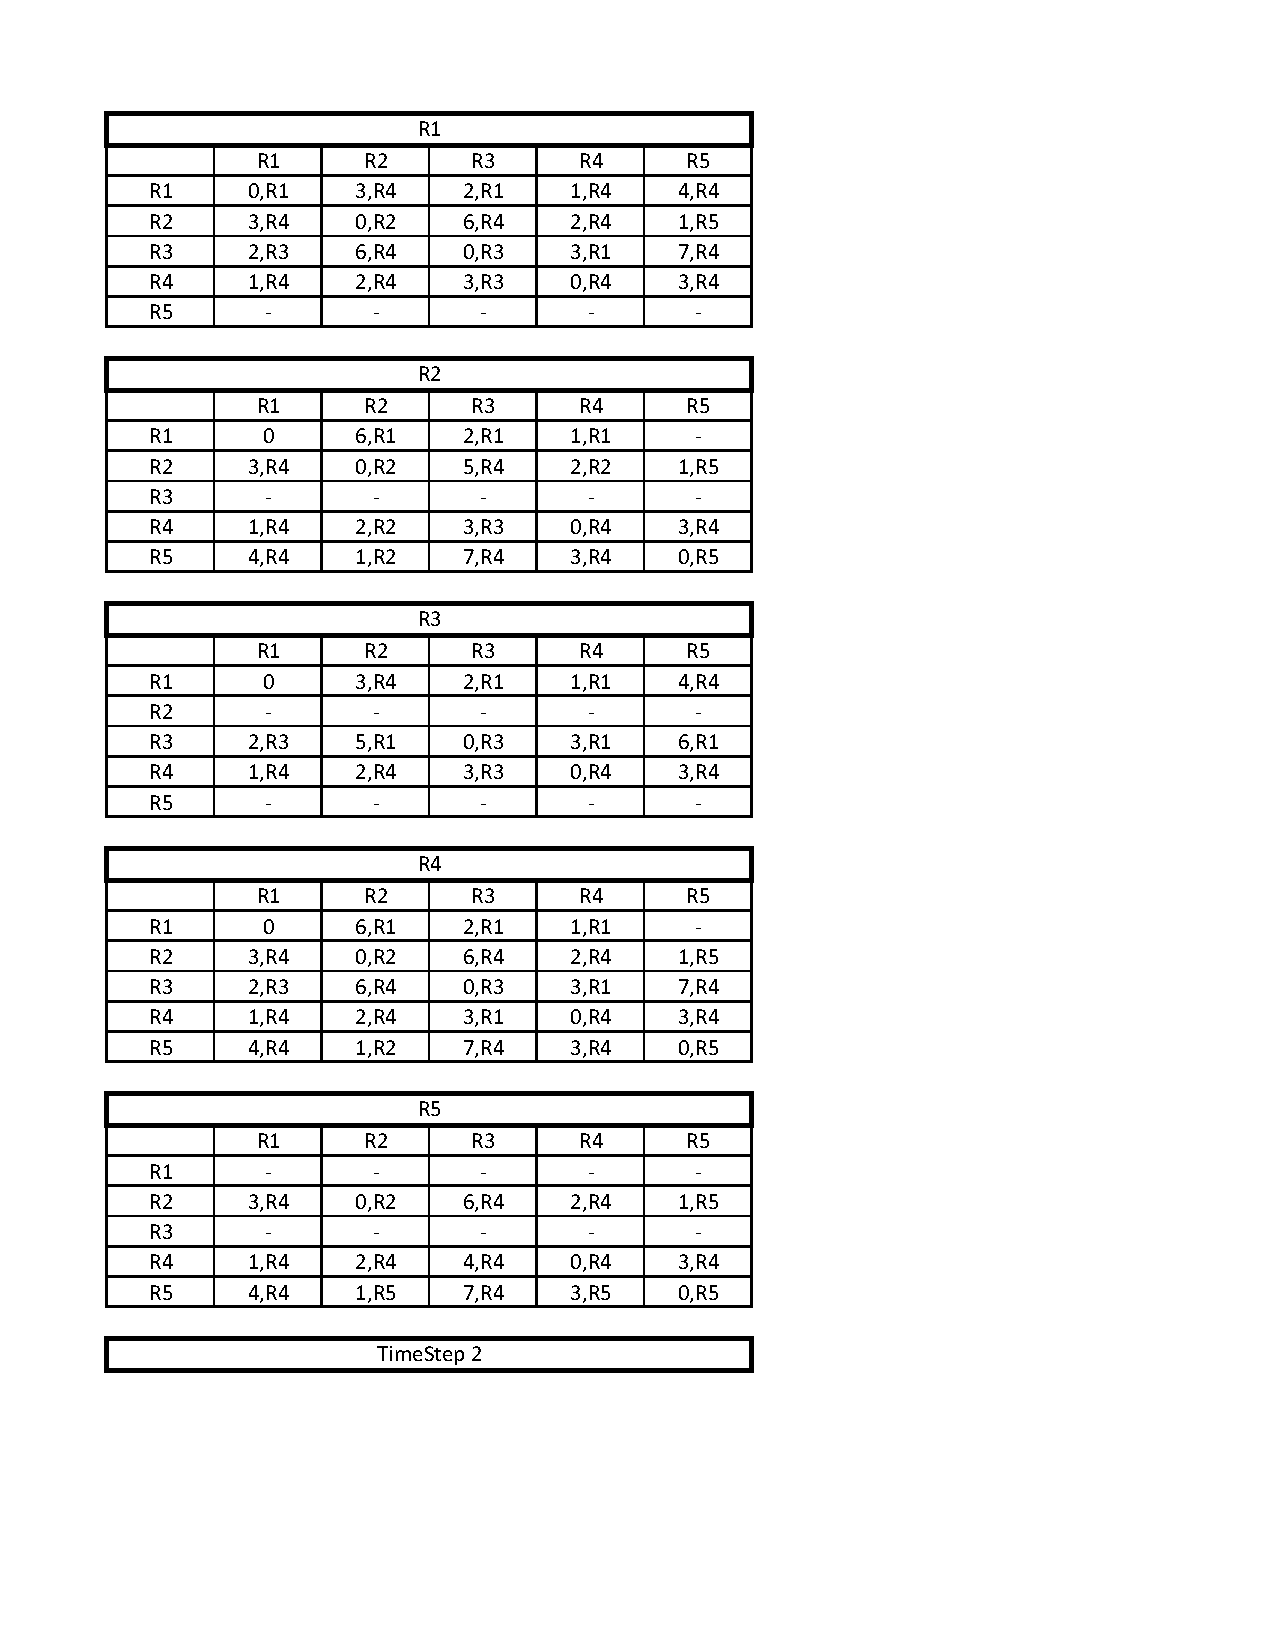
\includegraphics[width = 1.0 \textwidth]{images/3.pdf}
\end{center}


 \begin{center}
	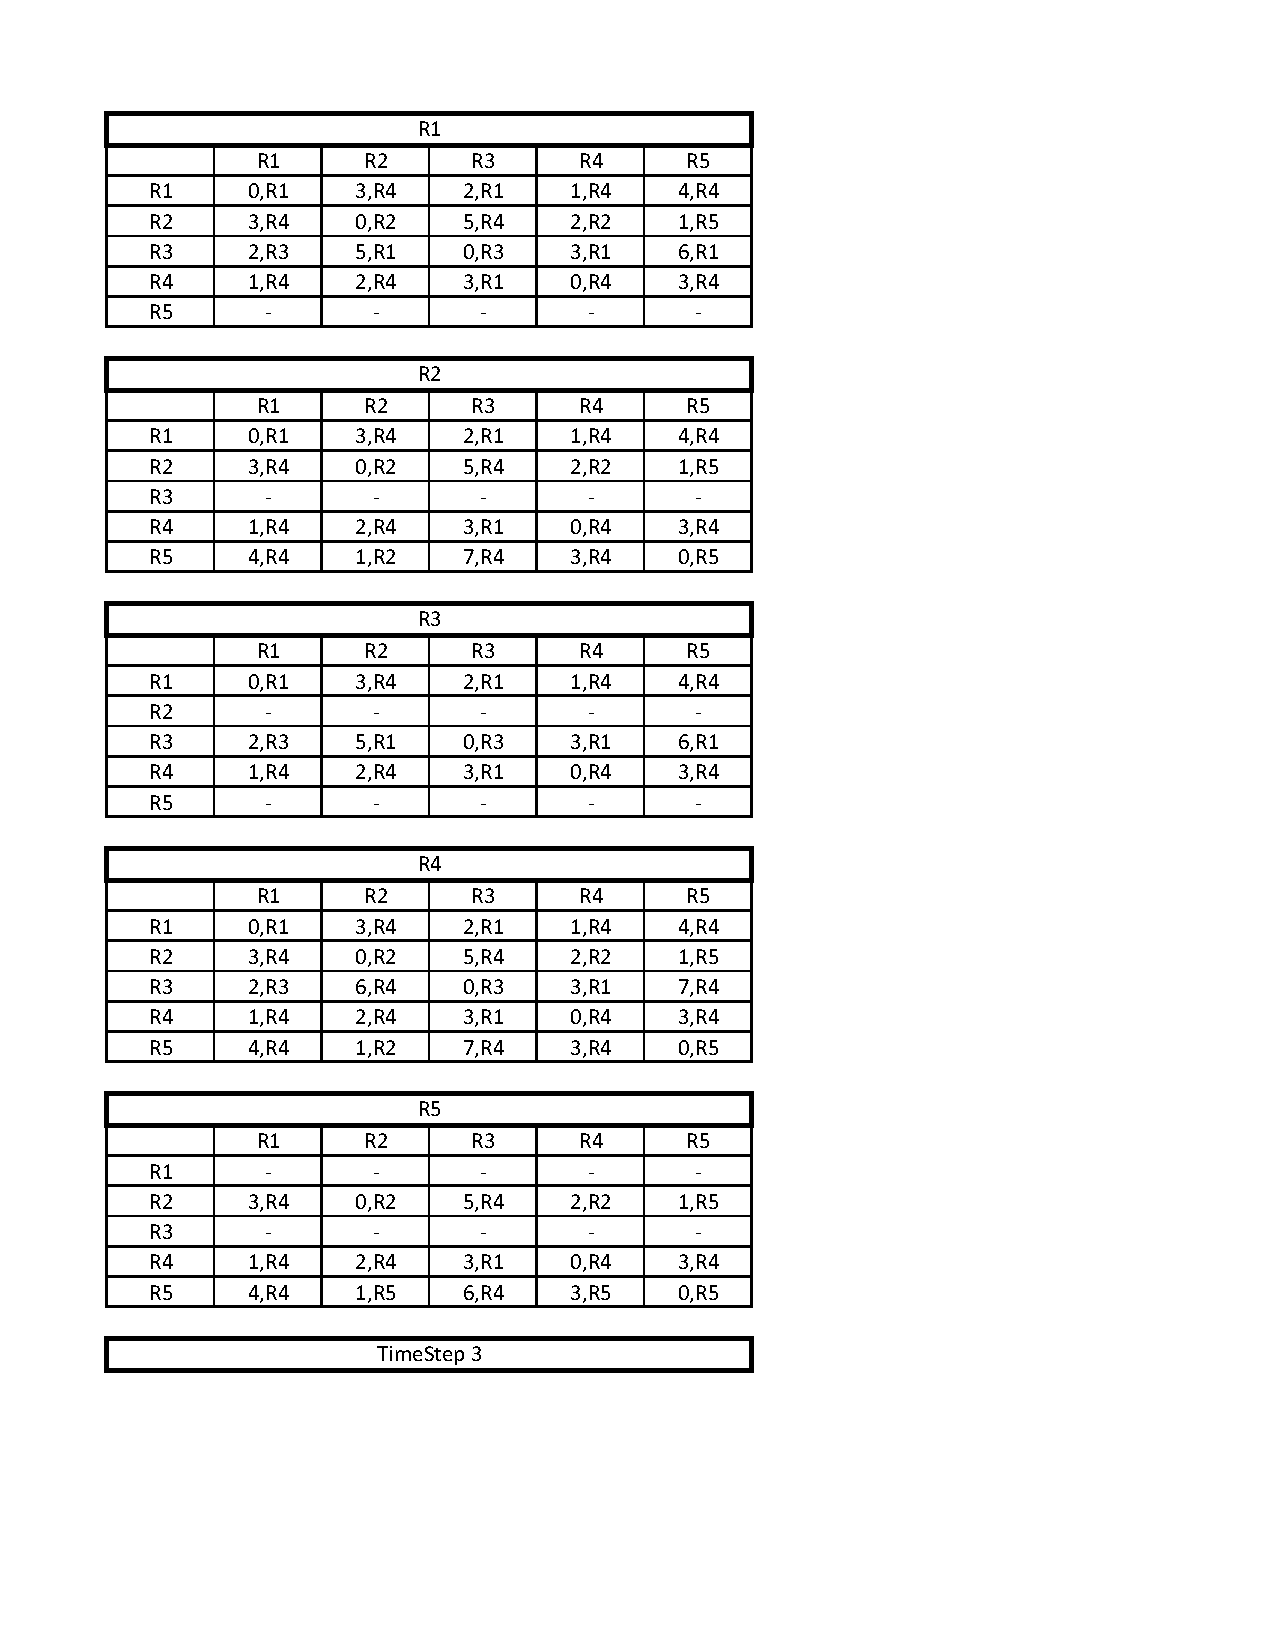
\includegraphics[width = 1.0 \textwidth]{images/4.pdf}
\end{center}


\subsection{RIP}


\begin{enumerate}[label = \alph*)]
	\item
	$$A\rightarrow D \rightarrow E$$
	
	\item
	$$C \rightarrow E \rightarrow D$$
	
	\item
	گراف شبکه به صورت زیر خواهد بود:
	
	
	\begin{figure}[h]
		\centering
		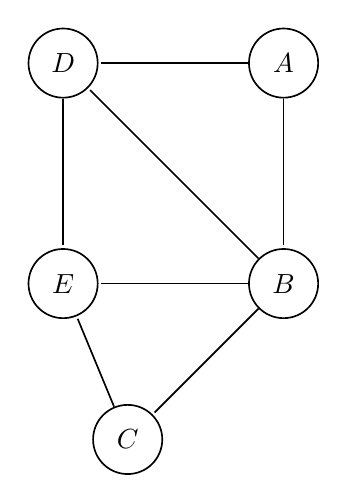
\begin{tikzpicture}[-,>=stealth',shorten >=1pt,auto,node distance=2.8cm,
			semithick]
			
			\node[state] (A)                    {$A$};
			\node[state] (B) [below of = A]                    {$B$};
			\node[state] (C)  [below left of = B]                {$C$};
			\node[state] (D) [left of = A]                    {$D$};
			\node[state] (E)     [below of= D]               {$E$};
			
			\path (A) edge  [above]   node {} (D)
			(A) edge  [above]   node {} (B)
			(B) edge  [above]   node {} (D)
			(B) edge  [above]   node {} (E)
			(B) edge  [above]   node {} (C)
			(C) edge  [above]   node {} (E)
			(D) edge  [above]   node {} (E);
					\end{tikzpicture}
	\end{figure}
	
\end{enumerate}

\end{document}



